\documentclass[12pt,a4paper]{book}
\usepackage[utf8]{inputenc}
\usepackage[inline]{enumitem}
\usepackage{parskip} % disable indentation for new paragraphs, increased margin-bottom instead
\usepackage[american,ngerman]{babel}
\usepackage{csquotes}

\usepackage{kit_style/kitthesiscover}

\usepackage[style=alphabetic]{biblatex}
\addbibresource{bib.bib}

\usepackage[%dvipdfm,
   pdfauthor={Christian Schwarz},
   pdftitle={Stage-aware Scheduling in a Library OS},
   pdfsubject={Bachelor Thesis},
   pdfkeywords={Operating Systems, Library OS, Scheduler, Cache-Affinity}
]{hyperref}

\usepackage{todonotes}
\usepackage{blindtext}

\usepackage{xparse}
\NewDocumentCommand{\sectionsubheading}{m}{%
    {\vspace{-0.7cm}\footnotesize #1 \vspace{0.25em}}\par%
}

\usepackage{xspace}

\usepackage{listings}

\lstdefinestyle{figurecpp}{
  belowcaptionskip=1\baselineskip,
  language=C++,
  basicstyle=\footnotesize,
  frame=single,
  xleftmargin=\parindent
}

\begin{document}
\frontmatter
\unitlength1cm
\selectlanguage{american}

\title{Stage-aware Scheduling in a Library~OS}
\author{cand. inform. Christian Schwarz}
\thesistype{ba}
\primaryreviewer{Prof.\ Dr.\ Frank Bellosa}
\advisor{M.\ Sc.\ Mathias Gottschlag}{}
\thesisbegindate{XX.\ December 2017}
\thesisenddate{XX.\ March 2018}
\maketitle

\begin{otherlanguage}{ngerman}
\thispagestyle{empty}
\vspace*{30\baselineskip}
\hbox to \textwidth{\hrulefill}
\par
\noindent Ich versichere wahrheitsgem"a"s, die Arbeit selbstst"andig verfasst, alle benutzten Hilfsmittel vollst"andig und genau angegeben und alles kenntlich gemacht zu haben, was aus Arbeiten anderer unver"andert oder mit Ab"anderungen entnommen wurde sowie die Satzung des KIT zur Sicherung guter wissenschaftlicher Praxis in der jeweils g"ultigen Fassung beachtet zu haben.\\

\noindent Karlsruhe, den \today
\end{otherlanguage}


\chapter{Abstract}
\chapter{Acknowledgments}

\mainmatter
\cleardoublepage
\phantomsection
\addcontentsline{toc}{chapter}{Contents}
\tableofcontents

\chapter{Introduction}
Network servers are of ever-increasing importance in today's cloud-based distributed infrastructure, handling requests from clients at high degrees of concurrency.
A common implementation pattern is a \emph{sequential} handler routine that processes each request, consisting of logical stages such as protocol handling, decoding/encoding and actual business logic.
Concurrency is achieved by executing the handler code per connection in separate operating system thread -- either by spawning a thread per request or by using a thread pool.
The sequential handler implementation is simple to follow for programmers and abstractions for the aforementioned threading models are available in virtually any programming language and operating system.~\cite{flashwebsrv,c10k}

Given the increasing CPU-memory-performance gap, it is paramount that the request handler's working set fits into the private CPU caches.
The instruction working set if of particular importance to feed the execution pipeline of contemporary super-scalar out-of-order processors.
The dominant CPUs in the server market are \texttt{x86\_64} based Intel processors targeted at the mass market.
The memory hierarchy of processors since the Haswell micro-architecture features separate 32KiB L1-d and L1-i caches and a unified 256KiB L2 cache per core, as well as a shared inclusive L3 cache that is significantly larger.\todo{ref}
However, recent large-scale profiling at Google suggests that this memory hierarchy fails to meet the demands of contemporary server applications:
request handling code exhibits little spacial locality and thrashes the private CPU caches, leading to sub-optimal branch prediction and pipeline stalls.\cite{kanev2015profiling}
%Hardware-supported operating system virtualization using KVM or Xen is commonly used to isolate applications both for simplified administration and increased security.
%Linux is the dominant guest operating system offering a familiar environment and high-performance paravirtualization drivers.

Previous work in this field includes techniques such as \emph{cohort scheduling}:
threads in the same working set are grouped into \emph{cohorts} and dispatched in series to reap the benefits of warm instruction caches.
If the shared working set fits into the cache for one series, instruction-dependent pipeline stalls are greatly reduced.
\emph{Staged Computation} expands this concept to general software architecture and \emph{staged event-driven architectures} (SEDA) generalizes it further:
request processing state is encapsulated into an object which is passed through a pipeline of stages interconnected by queues.
Each stage controls the concurrency model used to perform its work, allowing cohort scheduling to be employed.
A derivative of cohort scheduling has been implemented in a research DBMS under them term \emph{STEPS}, yielding an overall speedup of $1.4$ in the TPC-C benchmark.\cite{cohort,seda,steps,harizopoulos2005staged}

Despite promising results of above research, it has found little adoption in popular database management systems such as MySQL, which uses thread-based concurrency (one handler per request) with a pre-spawned pool of handler threads.~\cite{mysqlThreading}.
Furthermore, we find several assumptions in the designs of above solutions that no longer hold on today's SMP systems.
Therefore, we explore techniques that explicitly target multi-processor systems.
\emph{computation spreading} is a technique that splits the working set of thread at the user-kernel-boundary by executing OS code on different cores than user-level code, thus making use of the private caches more effectively.
Experimental work at the KIT OS group combines computation spreading with the idea of staged computation, resulting in a solution where
application developers manually partition their code into stages and inserts one-line stage switching calls into the request handling code path.
By dedicating CPU cores to stages and migrating threads between the cores on stage switch, the request handler's instruction working set is spread over the private caches of these cores.
A proof-of-concept implementation in Linux and the MySQL database management system show that i-cache misses and branch-misprediction rates can be reduced by X and Y\% respectively while keeping the modifications in MySQL to a total of just Z lines of C++.
However, experiments with multiple concurrent requests show that the prototype is not work-conserving on multi-processor systems.

This thesis shows that proper OS abstractions enable staged computation on modern SMP systems while requiring minimal customization effort in legacy applications.
Specifically, our contributions are as follows:
\begin{itemize}
    \item We analyze the design aspects that make the early 2000's approaches of cohort scheduling and STEPS inapplicable to SMP systems.
    \item We analyze the design and implementation of the aforementioned proof-of-concept implementation at the KIT OS group and point out why it is not work-conserving.
    \item We present OS abstractions and a user-space C++ API for applications to manually define stages and stage switching points in the request-handling code path.
    \item We present the design and implementation of a work-conserving scheduling policy that allocates CPUs to stages and migrates threads as necessary to preserve warm instruction-caches.
    \item We show that appropriate stage partitioning and switching points lead to a reduced cache miss rate of X\% in synthetic benchmarks and throughput gains of X\% in a stage-aware version of MySQL under the TPC-C benchmark.\todo{measurement}
\end{itemize}

The remainder of this thesis is structured accordingly.
In Chapter~\ref{ch:relwork}, we examine preceding work in the area of staged computation, including an analysis of their applicability to multi-processor systems.
Chapter~\ref{ch:analysis} dissects the KIT OS group's proof-of-concept implementation and points out why the design is not work conserving.
Subsequently, Chapter~\ref{ch:di} presents the design and implementation of our solution in the OSv library operating system.
Finally, we evaluate our implementation in Chapter~\ref{ch:eval}, using both synthetic microbenchmarks and the TPC-C benchmark against a stage-aware version of MySQL to show the intended cache behavior and performance improvements.


\chapter{Related Work}\label{ch:relwork}
High-performance network servers must handle requests at a degree of concurrency that exceeds the real parallelism provided by hardware in the form of CPU cores.
Much research has gone into techniques to handle this problem, further constrained by additional requirements such as predictable response times and fairness among clients.
This chapter starts with an overview of the prevalent concurrency models in the early 2000s' software landscape.
We proceed with an introduction to \emph{cohort scheduling}, \emph{staged computation} and \emph{staged event-driven architecture} which stem from the same time period
and present \emph{STEPS}, which applies above concepts to a research database management system, showing that these software-only solutions lead to performance improvements due to reduced i-cache misses and better branch prediction.
Despite these in reasearch systems, large-scale profiling at Google from 2015 shows that the memory hierarchy in contemporary processors is still sub-optimal for typical datacenter applications.
Given that the above approaches targeted single-core machines from the early 2000s, we take a step back and analyze their applicability to today's multi-processor systems and memory hierarchies,
coming to the conclusion that major redesigns are required in order to provide work-conserving solutions.
Motivated by the ongoing relevance of the topic and a changed hardware landscape, we explore \emph{computation spreading}, a technique that explicitly targets SMP systems and uses thread migration to spread the instruction working set of a thread over multiple CPU cores.
We conclude this chapter with a proof-of-concept implementation at the KIT OS group which extends computation spreading to arbitrary split points within user-level code, forming the basis for this thesis.

\section{Network Servers \& Concurrency}\label{ch:relwork:concmod}
% analysis of different htreading models with temrinology used in cohort scheduling: anderson paper
% better terminology can be foun din the SEDA paper
% see flash web server
% establish terminology like per-request threading, thread pool?
% flash web terminology => ours
% multi process / multi threaded = thread per request / thread pool
Network server software is generally concerned with receiving requests from clients over a network connection, acting upon them and returning a response.
In addition to the network I/O, disk access is very common, for example within file servers.
The request handlers are thus commonly I/O bound.~\cite{seda}

I/O \emph{hardware} interfaces are asynchronous, allowing the CPU to perform useful work while the slow I/O operation completes.
However, the traditional \emph{software} abstractions exposed by the operating system are synchronous:
processes or threads that \emph{block} on I/O operations are preempted from the CPU and only resume execution once the result of the operation is available.
Out of this situation, the following type of software architecture emerged:
\emph{multi-process} and \emph{multi-threaded} servers handle requests by following a sequential description of the steps involved to fulfill the requested task.
Concurrency is then achieved by having multiple threads (either spawned on demand or from a pre-spawned pool) execute the same request-handling function for different connections and to interleave these control flows by time-multiplexing the CPU.
This interleaving happens each time an I/O activity blocks or at the end of the scheduler-assigned time slice.
Canonical scalability problems with this approach are the context switching overhead and the minimal amount of memory each thread requires, e.g., for its TCB and stack.
Furthermore, synchronizing request handlers on shared resources without busy waiting requires kernel-supported synchronization primitives, implying syscall overhead.~\cite{flashwebsrv,c10k,andersonThreads,seda}

One alternative to the above are \emph{event-driven architectures} where the server consists of a loop that allocates a state object per request and implements a finite state machine driven by those objects.
Each thread of the server acts on one state object at a time, but does not perform blocking operations.
Instead, the operations are merely initiated and the state machine immediately switches to the next state object.
The server loop picks up the completion events of these asynchronous I/O operations and changes the corresponding state object accordingly.
This change in turn eventually triggers the state machine to perform the next logical request-handling step for the request represented by the state object.~\cite{flashwebsrv,seda,c10k}

For this thesis, the most relevant difference between multi-threaded and event-driven architecture lies in the representation of request-handling state:
multi-threaded servers encode it implicitly in the thread's execution state, consisting mostly of its stack, registers and instruction-pointer.
In contrast, event-driven servers explicitly define the finite-state machine and have a dedicated representation of the processing state in the state objects.

While the above description focusses on the role of I/O, nothing stops application developers from partitioning their CPU-bound or memory-intensive request-handling steps using the same mechanism.
The next sections give an introduction to \emph{staged computation} and \emph{staged event-driven architectures} which build ontop of the event-driven model.

\section{Cohort Scheduling \& Staged Computation}\label{ch:relwork:cohort}
In the early 2000s, \citeauthor*{cohort} investigated the cache behavior of I/O intensive online-transaction processing workloads (OLTP) in servers implementing the multi-process or multi-threaded architecture.
They observe high cache miss rates and instruction stalls, attributing it to the large amount of system calls made by the request handler threads:
system calls themselves have a large working set disjoint from the application code and may bring an entirely different working set into the cache when blocking and switching to another thread.~\cite{cohort}

\emph{Cohort scheduling} is then proposed as a scheduling policy to dispatch threads that are currently executing the same code segment in batches (\emph{cohorts}):
the first thread in a cohort may incur instruction / data cache misses but all successors of the same cohort benefit from a warm cache.
Naturally, the threads must yield the CPU before leaving this shared code segment and the segment size must not exceed the i-cache size to avoid thrashing the cache.
The size of a cohort represents the central trade-off in the scheduling policy: large cohorts yield fewer amortized cache misses but cause higher response time due to progress only being made once enough threads have reached the synchronisation point required for batch dispatch.
Furthermore, since the amortization only reduces the execution time but does not eliminate it, the minimum response time is necessarily increased.~\cite{cohort}

For immediate application, the authors suggest systems calls as pre-existing synchronisation points because they do not require modifying user-space code.
However, to increase cache locality in arbitrary parts of an application, the authors propose \emph{staged computation}:
in this programming model, instead of synchronous calls to subroutines, the request-handling stage posts asynchronous operation requests to other stages, each encapsulating a particular functionality and state.
A stage has \emph{scheduling autonomy}, which means it is free to choose the concurrency model that suits the type of provided operation best --- cohort scheduling being just one of several options.~\cite{cohort}.

Cohort scheduling at the syscall boundary is non-invasive with regards to application code bases and will we revisited by \emph{computation spreading} (Section~\ref{ch:relwork:compspr}).
In contrast, staged computation require non-trivial refactorings in existing applications, in particular if they already follow the multi-threaded model:
synchronous, blocking operations must be converted to asynchronous operations and continuations, and the scheduling autonomy granted to each stage must actually be addressed in code.

\section{Staged Event-Driven Architecture}\label{ch:relwork:seda}
% difference to staged computation: scalabiltiy, graceful degradation, no focus on cache locality
% formulation: control boundary, page 5 bottem right
% ease-of-use for application developers
% ref to cohort scheduling page 6 up left: example for auto-tuning of batrching factor (cohort size)
% give outlook on OS support for SEDA: specialized OS, no need for transparent resource virtualization as provided by threads
\emph{Staged event-driven architecture} (SEDA) is a software architecture generalizing the idea of staged computation.
The primary motivation for its inception was the construction of network services whose performance should degrade linearly under an increasing number of concurrent requests.
SEDA provides a framework for application developers to implement an event-driven server by only providing event handlers.
Each event handler represents a \emph{stage} and is invoked by its \emph{stage controller}, which executes the event handler on the stage's thread pool with input from the stage's \emph{incoming event queue}.
The event handler can enqueue additional work into other stages' queues, but cannot call into their code directly, enforcing an explicit boundary in the application's control flow.
The stage controller works in a feedback loop to ensure a stage's performance requirements, for example by adjusting the thread pool / \emph{cohort size} in order to meet a certain response time goal for event handlers.%
\footnote{SEDA terminology for a resource controller implementing cohort scheduling is \textquote{batching controller}.}
Stage controllers can coordinate to avoid resource over-commitment.
It cannot be stressed enough that the customizability of the stage controller is central to the whole concept of SEDA:
application developers are given control over the degree of concurrency and can address performance of code modules through custom stage controllers.~\cite{seda}

The authors evaluate SEDA by implementing an HTTP server and measuring the performance metrics \emph{total concurrent throughput} and \emph{response time} over a varying number of concurrent clients.
Additionally, they measure the amount of requests each client completes, defining an equal distribution of service among clients as ideally \emph{fair}. %Jain fairness factor
The results show 16--20\% higher throughput at little-varying response times and high fairness among clients in comparison to the the multi-threaded Apache web server. % leave out Flash, not interesting to us
The authors' explanation for these results is that the SEDA server queues all requests \emph{inside} the application while the multi-threaded Apache web server will not accept new client connections when reaching the maximum size of its thread pool, causing exponentially increasing response times for non-accepted clients due to exponential back-off algorithm employed in TCP.~\cite{seda}

SEDA shows the software-enginnering and performance benefits of staged computation.
In contrast to the proposal made in this thesis, SEDA requires fitting the application into the provided framework of event handlers and stage controllers.
This enables customizing the concurrency model and controlling resource usage \emph{per stage}, whereas our solution centralizes this functionality in the OS scheduler.
Notably, the SEDA authors suggest operating system support for their model, emphasized by their need to implement asynchronous I/O abstractions for their resource controllers.
While this may facilitate implementation of SEDA itself, it does not address the hurdle of refactoring existing code bases.

\section{STEPS}\label{ch:relwork:steps}
% split up dbms into stages by operators
% formulate the scheduling trade-off we found, too: response time vs cache efficiencey
% => make clear we handle this in our scheduling policy by balancing queue lenghts (i.e. adding more CPUs as necessary)
% in principle cohort scheduling, but with 'production line mode' in mind, this is (not exactly what we do, in theory stages can be entered again...)
% come to conlcusion that staged system must have dedicated CPUs per stage (p10, 5.3 intro)
% use ults to switch between threads in a cohort (3.3.1):
% p8 rechts oben: threads executing same db operation are grouped into teams of so called S-threads, linked in doubly-linked list. at ctx, switch to next entry in linked list => fast, high hit rates
%                 when an S-thread blocks (yields the CPU), it leaves that team (stray thread)
% p9: data-dependnet teams where overalp between S-threads is not big enough
% p9: trick for blocking / yielding threads:
%       1. intercept block events, remove blocking thread from team list, hint to "regular" (=OS/thread package) scheduler next thread in team-list should be run, continue blocking, will schedule team-list memeber
%       2. (rechts unten): nur wenn man keine mutex hält wird gescheduled, sonst nicht, weil dann die ganzen anderen thread snicht weiterkommen
%       => THEY HAD THE SAME PROBLME WE HAD!
%       => section 4.1.4 reads like they did all modifications to the DB, nothing reusable in other applications

% paper review:
% 3.1 "Most commercial DBMS involve a light-weight mechanism to pass on CPU control (Shore uses user-level threads)." (trifft bspw. auf MySQL nicht zu)
The \emph{Synchronized Transactions through Explicit Processor Scheduling} (STEPS) project implements a derivative of cohort scheduling in the research database system SHORE.~\cite{shore}

The authors replicate the observation of \cite{cohort} for database systems: the execution flow exhibits low spatial locality and do not fit into the CPU caches, leading to pipeline stalls and a high amount of mispredicted branches.
In contrast to cohort scheduling, STEPS groups threads handling a transaction into \emph{team lists} organized by high-level operation (e.g., \texttt{\textsc{insert}}, \texttt{\textsc{update}}.
The code path of the operation then contains context-switching points (\textit{\texttt{CTX} calls}) at which the currently executing thread yields control to the next member of its team list, which amounts to user-mode round-robin scheduling within a team.
Context-switching points are placed such that the working set between two of them fits into the CPU's L1 i-cache.
The idea of cohort scheduling is found in the step-by-step progression over the long code path of the high-level operation:
we imagine three contex-switching points $A$, $B$ and $C$ and a team of ten threads executing between $A$ and $B$, operating on a fully utilized warm i-cache.
After the last thread reaches $B$, the team moves forward to the next step  \textit{$B$ to $C$}.
Although the first thread executing this step will incur capacity i-cache misses, it pre-warms i-cache and branch predictors for the remaining nine threads.~\cite{steps}

\begin{figure}[h]
    \centering
    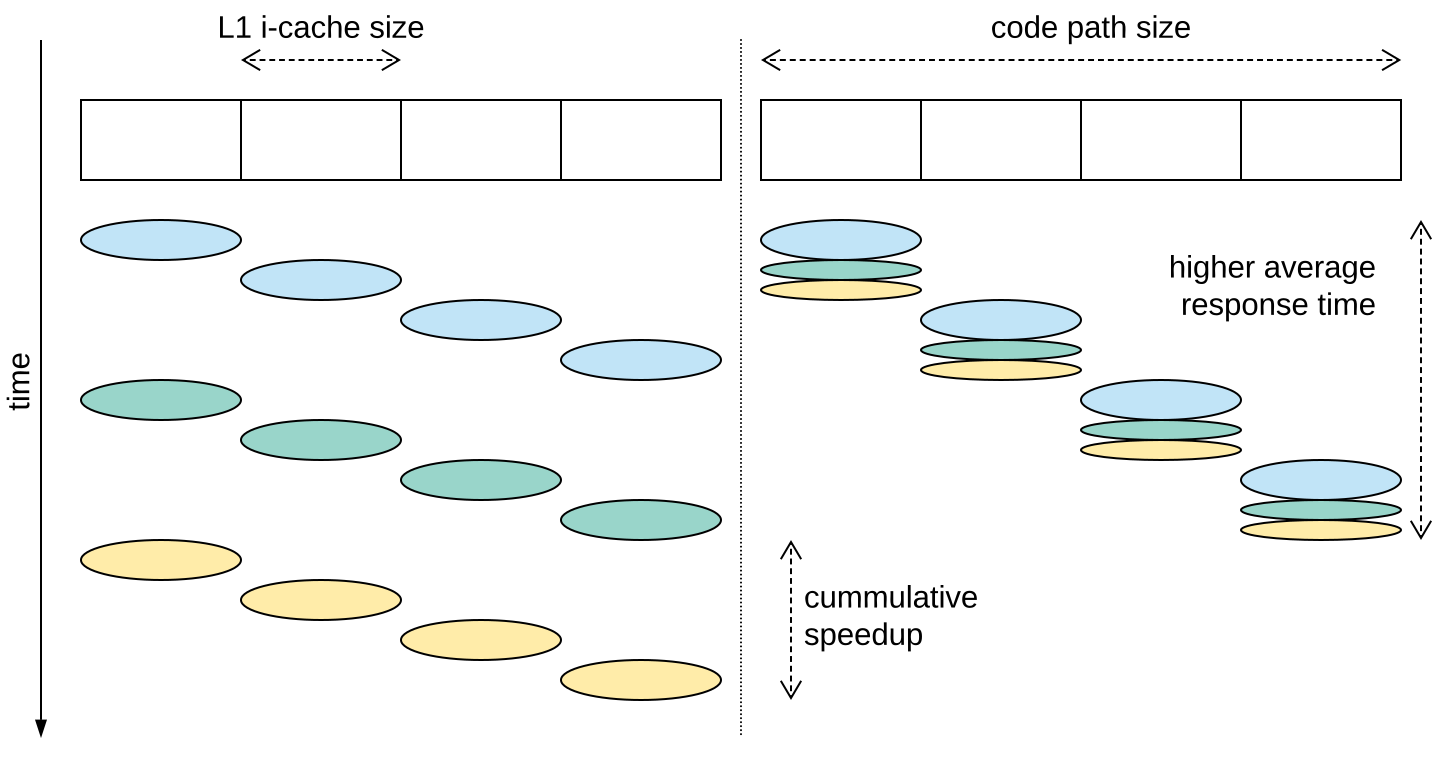
\includegraphics[width=0.8\textwidth]{fig_build/cohort_and_steps.pdf}
    \caption{
        Idealized scenario of three threads (different colors) executing the same code path that does not fit into the L1 cache.
        \textbf{Left}: each thread passes through the code completely before yielding CPU to the next thread.
        \textbf{Right}: team of threads trickles down the code path in code segments that do not exceed the L1 i-cache size.
    }
    \label{fig:cohort_and_steps}
\end{figure}

Blocking threads or threads aborting the transaction, would fall behind in this trickle-down schema and thus replace their ex-team members' cache state.
The solution is to remove threads aborting their transaction or blocking for synchronization and I/O from the team list and track them as \emph{stray threads}.
The publications on STEPS describe that the thread package in SHORE required modification to support this schema, but falls short on implementation details.
For this thesis, though, blocking is a highly relevant topic because it is a major problem in the proof of concept implementation at the KIT OS group (see Section~\ref{ch:relwork:kitpoc} and Chapter~\ref{ch:analysis}).
By examining the 6.0 release of SHORE which was published after STEPS, we can identify a base class for all DBMS threads called \texttt{sthread\_t} which provides wrappers for basic blocking I/O functions such as the \texttt{read} or \texttt{write} syscalls.
%Under the assumption that these abstractions existed in the version of SHORE that STEPS is based on, we can imagine that they were used to get notified about potentially blocking I/O requests by a thread in order to remove it from the team list.
%However, such an approach would not be able to differentiate between an actual block vs. non-blocking retrieval from the page cache and thus cause avoidable collateral damage to the thread requesting I/O.
%On the other hand, the code footprint of the I/O path could evict the team's working set from the cache --- an argument in favor of indistinguished removal from the team if I/O is pending.
Under the assumption that these abstractions existed in the version of SHORE that STEPS was based on, we are confident that the STEPS authors used these wrappers to get notified about potentially blocking I/O requests by a thread in order to remove it from its team list.~\cite{shoreRelease,shore}

Regardless of the exact implementation details, we are not convinced that the adoption of STEPS in arbitrary applications requires as few code modifications as claimed by the authors:
SHORE already comes with a custom thread abstraction around pthreads and centralized wrappers around blocking I/O.
In contrast, arbitrary applications will use the pthreads and C standard libraries directly, in which case
either substantial modifications to the code base are necessary to establish a situation as found in SHORE
or runtime-patching via \textsc{\texttt{ld\_preload}} would be required.

Lastly, STEPS's handling of stray threads should be considered: recall that stray threads are removed from their team when performing potentially blocking syscalls, and only re-join a team when being re-used for a new high-level operation.~\cite{steps}
Specifically, this means that STEPS does not account for the instruction footprint of the operating system at all.
However, \citeauthor*{osCacheFootprint} show that the operating system has a significant cache footprint and should thus be considered when trying to optimize the i-cache footprint.~\cite{osCacheFootprint,compspr} % osCacheFootprint: summary
Another perspective on the situation is that stray threads will continue to compete for CPU time for the time they are not blocked.
Since the OS scheduler is unaware of the team lists, it may schedule a stray thread in the midst of a team, evicting its cache state inadvertently.
STEPS tries to prevent this by giving a \textquote{hint} to the scheduler to prioritize the next thread that remained in the team, but does not elaborate on the additional syscall overhead.
By proposing a solution that is rooted in the OS's scheduler, we avoid the information loss and implementation complexities associated with STEPS's user-space approach.

\section{Profiling Datacenter Applications}\label{ch:relwork:profiling}
% alread shown that it's a problem in DBMSs, see 'affinity scheduling harizopoulos introduction' and the Steps paper (p3)
% dominant are the d-cache misses, but i-cache misses are also significantly higher than usual 
% growth of i-cache working set over time (speculation: due to product development) => worsens situation
% => stall cycles, X %
% memory latency, not band width

% TODO https://software.intel.com/en-us/vtune-amplifier-help-front-end-bound
While the micro-architectural performance problems caused by large i-cache footprints were already observed in \cite{cohort} and \cite{steps} in the early 2000s,
recent profiling work at Google shows that computer architecture is still not able to satisfy the requirements of contemporary scale-out applications.
However, the potential performance gains and cost savings due to improved cache behavior become relevant at scale, motivating a re-assessment of the situation.

\citeauthor*{kanev2015profiling} identify a significantly higher amount of pipeline stalls in real-world datacenter applications when compared to the SPEC CPU2006 benchmark.
Apart from the overhead associated with the distributed software architecture (RPC, serialization, etc) % datacenter tax
a large cache footprint (both code and data) reveals the major performance bottleneck on today's processors for typical datacenter applications:
the authors observe 60\% of $\mu$op slots to be backend-bound, and 15 -- 30\% to be front-end bound, which leads to heavy under-utilization of the CPU cores' available resources at a micro-architectural level.\todo{do not require pre-existing knowledge about arch}
In particular, the authors find that more than 5\% of cycles are wasted due to empty front-end buffers, which is attributed to instruction read misses in the private L2 cache, resulting in slow accesses to the CPU's shared last level cache.
Additionally, the observations confirm that applications under active development grow in their instruction working set, worsening the situation.%
\footnote{The authors present exemplary results of up to 27\% per year.}
The authors do not explicitly investigate why datacenter applications have such large instruction working sets but mentioning \textquote{lukewarm} code and static linking as possible contributors.~\cite{kanev2015profiling}

In comparison to the work published a decade earlier (see Section~\ref{ch:relwork:cohort}~and~\ref{ch:relwork:steps}),
\citeauthor*{kanev2015profiling} focus on computer-architecture and only pay brief attention to the operating system:
approximately 20\% of CPU time is spent in the kernel with more than 5\% of CPU time in the scheduler alone.
Additionally, it is noteworthy that a 90-th percentile of the observed machines handles more than 4500 concurrent threads.
Given that at least a portion of these threads will be part of network servers, the question of the concurrency model thus stays very relevant although not explicitly stated as a source of performance-optimizations.~\cite{kanev2015profiling}

Looking at the related work presented so far, we conclude that for more than 15 years, typical datacenter applications have been observed to exhibit high i-cache-miss and branch-misprediction rates, resulting in sub-optimal use of the available CPU resources and motivting continued research in this field.

\section{Interim: Applicability to SMP Systems}\label{ch:relwork:anasmp}
Cohort scheduling, SEDA and STEPS were all evaluated on single-core machines.
Adaption to multi-core systems is not mentioned at all or stays theoretical.~\cite{steps,harizopoulos2003case}
Given today's ubiquitous multi-processors and the ongoing relevance of high i-cache footprints, re-examining the applicability of the above approaches seems appropriate.

\subsection{Private Caches}
% All numbers by example: My Haswell against STEPS CPU
% L1 and L2 are now oncore, L3 is shared (and inclusive on Intel)
% In contrast: early 2000s processors were single-core, L1 and L2
% capacities of L2 now what we have in L2 on-core
% today's L1 is split 32KiB i- and d-cache, early 2000s L1 64KiB (shared / unified?)  
% proof that today's chips are multicore: begin sodaspr
The single-core machines used to evaluate cohort scheduling, SEDA and STEPS feature a small L1 cache and a larger, higher-latency L2 cache.
However, contemporary symmetric multi-processors typically have a \emph{private} L1 and L2 caches and a \emph{shared} L3 cache.
The capacities of L1 and L2 are comparable to the early 2000s' models and the access latency between L1, L2 and L3 increases by a factor of 3 -- 4 between each level.
However, L2 instruction misses can typically not be compensated by out-of-order processing.~\cite{hennessy2002,haswellCacheLatency} %hennessy print page 509

An adaption of cohort scheduling and STEPS to multiprocessors must thus target the private caches of each core to achieve the similar benefits.
More importantly, the existence of private caches per hardware thread introduces the problem and opportunity to allocate this resource:
in terms of STEPS, multiple steps can now be spread over different cores instead of time-multiplexing the single available L1 i-cache.
We come back to this observation when assessing \emph{computation spreading} in Section~\ref{ch:relwork:compspr}.

\subsection{Real Parallelism}
We recall from Section~\ref{ch:relwork:cohort} that the scheduling trade-off in both approaches consists of reduced cache misses vs. increased response time due to \emph{batching}.
However, the real parallelism available on SMP systems brings with it another scheduling dimension that STEPS and cohort scheduling do not address:
to utilize the available hardware threads, load must be balanced among them to maximize resource utilization.
This goal surpasses response time since as the primary scheduling goal since the the service provider generally pays for the number of cores, not their actual usage.\todo{well actually... cpu time accounting}
All relevant operating systems abstract CPU cores through threads, and the OS scheduler implements load balancing by migrating threads between cores, often directed by metrics such as the length of each core's the ready queue (\emph{load}).~\cite{freeBSDSchedulerLoad}

Cohort scheduling and STEPS were not designed for this situation because
%both solutions include \emph{batching} as a central element, either at the syscall boundary or at arbitrary points in the application code (see Section~\ref{ch:relwork:cohort}~and~\ref{ch:relwork:steps}).
\textbf{batching is inherently not work-conserving on SMP systems}:
all threads in a cohort or team must run on the same core in order to benefit from the warm i-cache, but this means only one thread per team can run at any given time.
Furthermore, STEPS and the OS scheduler work actively against each other because the latter will see all threads in a cohort as runnable and actively spread the cohort over all (presumably idle) cores,
destroying all promised performance benefits.

An easy fix would be a mechanism for STEPS to influence the load balancing in order to favor threads of the same team to stay on the same core, e.g., through thread pinning.
This is obviously not work-conserving on multi-core systems, requiring additional mechanisms and communication between STEPS and the OS to fix it.
On a busy system, one could also argue that enough threads are available to simply employ cohort-scheduling per core.
However, in contrast to the approach of \emph{computation spreading} presented in the next section, this replicates to each core the repeated capacity misses when a team moves to the next step.

The above assessment shows that cohort scheduling, SEDA and STEPS cannot be directly applied to today's multi-processor systems.
The availability of private caches per core must be accounted for and new requirements such as load balancing between cores must be addressed.
However, given the ongoing relevance of the problems identified more than 15 years ago, we continue this chapter by investigating publications that explicitly target multi-processor systems.
\todo{s/multi-processor/multi-core/?}

\section{Computation Spreading}\label{ch:relwork:compspr}
% TODO: related and actually more relevant to our approach: Computation Spreading
% => term: destructive interference
% => migration for syscall => split i-working set (naturally) + little communication (because sendfile)
\emph{Computation spreading} (CSP) in its most general form is a technique to cache the instruction working set of a process more effectively on SMP systems which commonly feature private caches per core.
\citeauthor*{compspr} show that this cache hierarchy leads to redundantly stored code.
For example, in a traditional thread-based concurrency model, each request-handling thread may interact with the file system through system calls which leads to redundantly stored file system code being in each core's private cache.
The authors present a solution that temporarily assigns CPU cores to either execute OS code or user-level code, exploring and evaluating several allocation policies.
Threads entering or leaving the OS synchronously through syscalls, exceptions or page faults are then migrated between compatible cores.~\cite{compspr}

A central aspect of the implementatio is the thread migration mechanism which is based on hardware virtualization features:
all synchronous kernel entries are intercepted and used to trigger the thread migration, leaving the \textit{guest} OS and user-space software completely unmodified.~\cite{compspr}
An easy-to-overlook detail however is that the hardware-based thread migration is only available in hypervisor mode, which means that cooperation from the software executing in this mode is required.
Deployment in public clouds based on hardware-virtualization is thus only possible with explicit support by the cloud provider and would thus require further work in the hypervisor scheduler.
Our solution does require hardware virtualization due to limited driver support but implements thread migration in software and can thus be deployed to existing infrastructure.

The authors evaluate their solution using full-system simulation of an eight-core machine with private L1 and L2 cache and a shared L3 cache.
Server applications, which are of primary interest for this thesis, exhibit 25 -- 58\% fewer L2 instruction misses and 9 -- 25\% improved branch misprediction rates.
Data read misses are less affected, with only 13 -- 19\% decrease for Apache web server and an OLTP application.
The approach leads to a speed-up of up to 20\% in Apache and 9.4\% in OLTP measured by the total runtime of the full-system simulation.~\cite{compspr}

Despite the very specific implementation, it should be noted that the concept presented by the authors is more general and not limited to the syscall interface:
they suggest migration points at arbitrary positions in the application code and corresponding core allocation policies.~\cite{compspr}
However, we cannot find a proposal to implement this, which is a very welcome segue to the next section.
\todo{hardware-based approaches?} % http://ieeexplore.ieee.org/document/1410076/

\section{Prototype in Linux at the KIT OS Group}\label{ch:relwork:kitpoc}
%TODO this section should coin the term stage-aware scheduling, otherwise, we need to do that before the analysis --- rename section with stage-aware in title
\NewDocumentCommand{\klt}{}{\textsc{klt}\xspace}
\NewDocumentCommand{\klts}{}{\textsc{klt}s\xspace}
\NewDocumentCommand{\ult}{}{\textsc{ult}\xspace}
\NewDocumentCommand{\ults}{}{\textsc{ult}s\xspace}
A Linux-based proof-of-concept implementation at the KIT OS group combines the idea of staged execution, cohort scheduling and computation spreading into a C API that allows for intuitive conversion of existing code bases to staged execution:
the application developer manually identifies stages and inserts library calls into application code for switching the current stage.
Each CPU core is assigned one or more stages and each time a thread switches to a new stage, it is migrated to a core assigned to that stage, benefiting from a warm i-cache.
Obviously, this approach targets applications that employ thread-based concurrency, i.e. the multi-threaded server architecture outline in Section~\ref{ch:relwork:concmod}, since the stage-switching is embedded into the control flow of the request handler and thus not explicitly modeled like in SEDA (see Section~\ref{ch:relwork:seda}).

Fast thread migration mechanism is required for this technique to succeed
--- otherwise, the performance benefits of always-warm caches per stage are destroyed by the migration time.
%\newcommand{\setaffinity}{\texttt{sched\_setaffinity(2)}}
The Linux built-in facility for this purpose, \texttt{sched\_setaffinity}, is impractical because it uses
expensive inter-processor-interrupts to implement this syscall, resulting in $9\mu s$ -- $14\mu s$ of migration time.
As a consequence, thread migration was implemented in user-space:
for each user-level thread (\ult), there still exists exists a kernel-level thread (\klt),
but \klts are pinned once to a specific core and stage.
\ults run on a \klt of the stage they are currently in and migrate to a different \klt when switching stages.~\cite{sodaspr}% sodaspr:table 1

When a \ult makes a call to switch stages, its context is saved and enqueued into the next stage's incoming migrations queue.
The originating \klt now waits for new \ults on its own stage's incoming migrations queue.
If it is empty, the \klt makes a blocking syscall \texttt{sys\_dequeue} to a kernel component to wait for incoming migrations.
The kernel component must ensure that there is always one \klt per core either doing work or actively dequeuing \ults in order to utilize the CPU.
This is implemented by a callback from the Linux scheduler that informs the kernel component of task state changes.
For example, if the currently dequeuing \klt $K_1$ executes a \ult, and that \ult blocks on a mutex, $K_1$ transitions from \texttt{running} to \texttt{blocked}.
The kernel component must wake up another \klt $K_2$ that is currently waiting for incoming migrations of that stage on that core.
Otherwise, the core does not perform any work (for the application) until $K_1$ acquires the mutex and becomes \texttt{runnable}.
Figure~\ref{fig:kit_os_poc_blocking} visualizes this situation.

\begin{figure}[h]
    \centering
    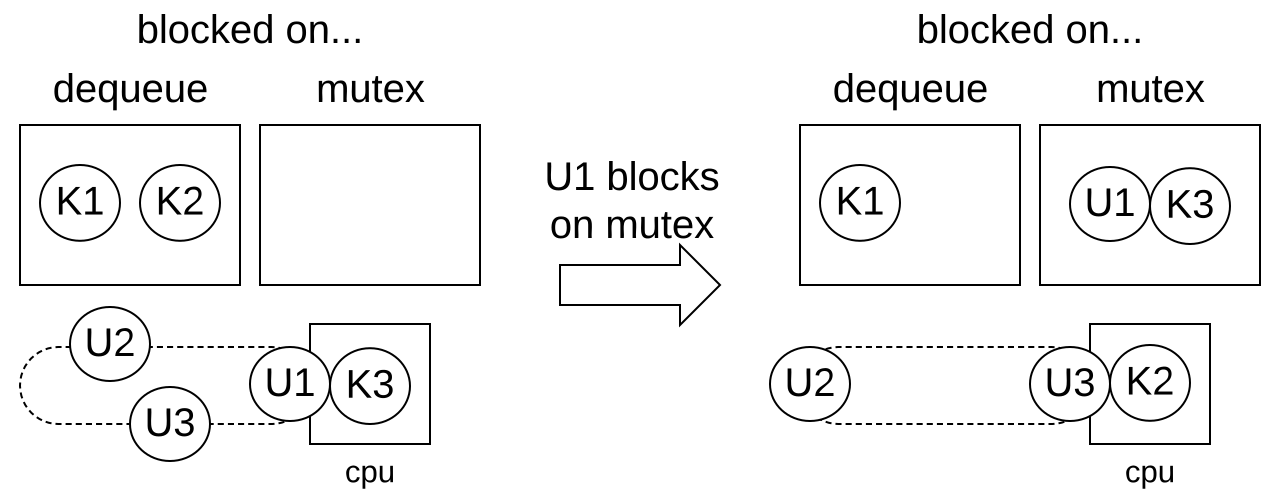
\includegraphics[width=0.8\textwidth]{fig_build/kit_os_poc_blocking.pdf}
    \caption{When a \ult issues a blocking syscall, the current \klt blocks. Another \klt must take over executing \ults from the core's queue. Note that while there is a \klt for each \ult, the relationship is not fixed.}
    \label{fig:kit_os_poc_blocking}
\end{figure}

The authors evaluate their design with microbenchmarks and performance-counters, showing x\% fewer i-cache misses, y\% fewer mispredicted branches.
Additionally, a full-system evaluation is made by comparing the benchmark results of the TPC-C OLTP benchmark on Linux 4.X between an upstream and a \emph{stagified} version of MySQL 5.6.38 running on an SMP system with X cores.
The expected reductions of i-cache and mispredicted branches are achieved in the stagified version, but overall throughput depends on the number of concurrent requests.
taking upstream as baseline (100\%), throughput with a single TPC-C terminal is z\% higher in the stagified version, but multiple terminals and thus concurrent requests leads to Z2\% of upstream's throughput.
The proof-of-concept is thus clearly not work-conserving on SMP systems, which we will investigate in the next chapter.
\todo{data}

\chapter{Analysis}\label{ch:analysis}
Related work has demonstrated that spreading the working set of an application over multiple cores yields lower on-core cache miss rates.
The proof-of-concept implementation at the KIT OS group furthermore shows that large-scale refactoring of existing code bases is not necessarily required to spread the working set:
given an application with a suitable threading model, patches of a few lines are sufficient to reduce i-cache misses and branch-misprediction significantly.

However, its evaluation on an SMP system shows that the solution is not work-conserving as visualized in Figure \ref{fig:kit_os_poc_work_conserving}:
imagine a system with multiple cores per stage and a \ult $U_1$ in stage $S$ executing on a \klt $K_1$.
As described above, $K_1$ is pinned to core $C_1$.
When $U_1$ performs a blocking syscall, for example when trying to acquire a lock, $K_1$ blocks.
The Linux scheduler now dispatches another task $T$ on $C_1$ to maximize CPU utilization, where $T$ is not a $K_i$ of our application.
In fact, all $K_i$ are blocked in \texttt{sys\_dequeue}.
When $K_1$ finally acquires the mutex and is \texttt{ready} again, it is still pinned to $C_1$ because the solution needs this to perform thread migration in user-space.
However, $C_1$ is still executing $T$, not $K_1$, and thus $K_1$ must be put into $C_1$'s ready queue.

The problem at this point is that there may exist \emph{another} CPU $C_2$ where a \klt $K_2$ is dequeuing \ults in the \emph{same stage} $S$:
if $K_2$ does not have any \ults to execute, $K_1$ should be migrated to $C_2$ immediately when it is woken up and continue execution there, benefiting from the warm on-core caches.
But the implementation only performs thread migration when a \ult calls the stage switching API.
There is no mechanism in place to save $K_1$'s state and enqueue it to $K_2$'s incoming migration queue on wake-up.
One might assume it is possible to enqueue $U_1$ to $K_2$ since we saved its register state on kernel entry via \texttt{pthread\_mutex\_lock}:
this is not possible because there might still be kernel code that needs to run after the mutex is acquired, before returning to $U_1$.

\begin{figure}[h]
    \centering
    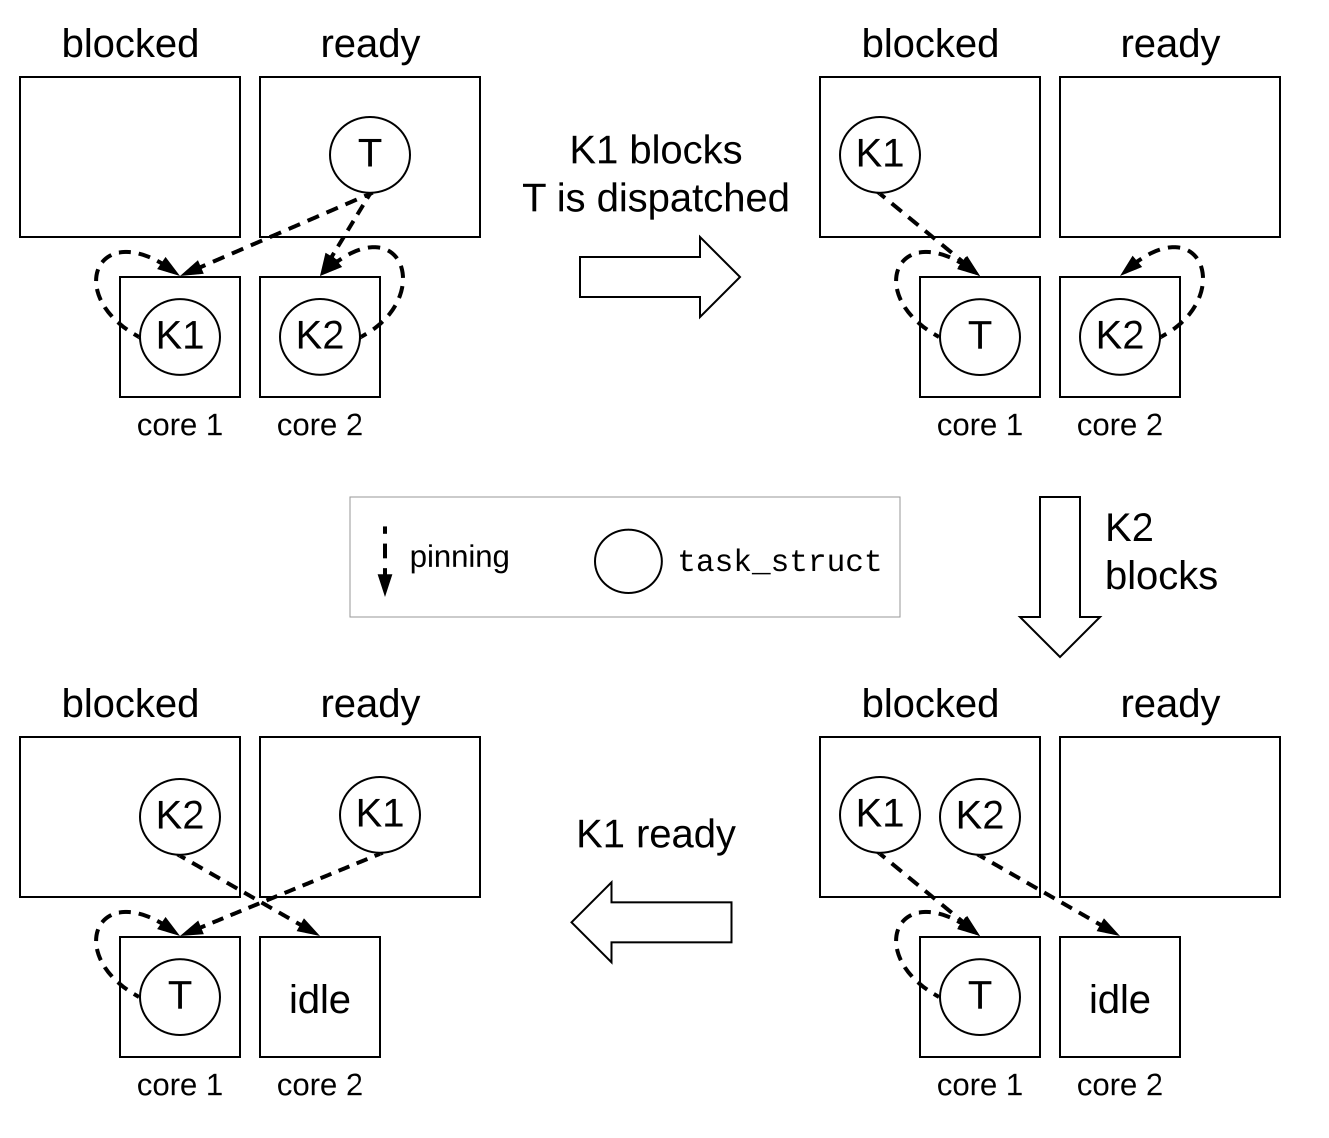
\includegraphics[width=0.8\textwidth]{fig_build/kit_os_poc_work_conserving.pdf}
    \caption{The proof-of-concept implementation is not work-conserving. When K1 becomes ready it should be dispatched to C2 immediately. But K1 is pinned to C1 due to the implementation of thread migration.}
    \label{fig:kit_os_poc_work_conserving}
\end{figure}

We identify several fundamental problems in the approach taken by the proof-of-concept implementation:
the requirement for fast thread migration drove the design toward a user-space solution which decouples the threads known by the application (\ults) from the threads known by the kernel (\klts).
However, the kernel scheduler still only handles \klts and assumes a 1:1 threading model, which leads to an \textbf{ambiguous role of \klts} in the proof-of-concept:
when switching between stages, the user space thread migration code views \klts as the CPUs they are pinned to.
But when a \ult running on a KLT interacts with the Linux kernel, the kernel sees a normal \texttt{task\_struct} and continues to assume the 1:1 threading model where tasks can just block.
The proof-of-concept works around this schizophreny by introducing a callback from the scheduler to react to blocking \klts, but fails to handle asynchronous events like wake-ups.
The latter leads to non-work-conserving behavior on multi-core systems.

We conclude that the proof-of-concept does not model the situation correctly: the association of stages and CPU cores is piggybacked onto the \klts using \texttt{sched\_setaffinity}, leading to an ambigous role of \klts.
We thus propose that stages must be modeled explicitly in the kernel and be separate entities, beneath CPUs and threads:
\begin{itemize}%
    \item The association of stages and CPU cores must be represented explicitly.
    \item Threads must carry the information in which stage they are executing.
    \item The scheduler must honor this information by scheduling threads onto cores that are associated with their respective stage.
    \item The scheduler must trade off the potential gains of always-warm caches against existing scheduling goals such as resource utilization, fairness and response time.
\end{itemize}%
This reverts the complex situation of \ults and \klts to a simple 1:1 threading model, removing the special-case of blocking kernel activity.

The remainder of this thesis presents our design as well as its implementation in the OSv library operating system and the evaluation using microbenchmarks and the TPC-C benchmark with MySQL.\todo{repetitive?}

\chapter{Design \& Implementation}\label{ch:di}
Certain classes of datacenter applications exhibit large instruction working sets that do not fit into the private cache of commodity processors.
On a micro-architectural level, this leads to underutilization of the cores' available computing resources, and thus worse application performance.
This chapter presents our operating-system-based solution to mitigate this problem in multi-threaded servers which handle client connections in threads, each following the same, sequential, potentially blocking, code path.

For example, in a database management system that is accessed over TCP, a request-handling thread will
\begin{enumerate}[label=(\alph*)]
    \item read the request data from a socket, using the network stack, \label{en:di:ov:read}
    \item deserialze \& parse it, \label{en:di:ov:des}
    \item perform the requested operation,\label{en:di:ov:processing}
    \item serialize the response and \label{en:di:ov:ser}
    \item send it back to  the client. \label{en:di:ov:write}
\end{enumerate}
While not true for all types of servers, database systems for example exhibit a a significant i-cache footprint in step~\ref{en:di:ov:processing} per high-level SQL operation (see Section~\ref{ch:relwork:steps}).
The code footprint of the network stack is also significant, as is the filesystem and potentially the serialization library.

All these steps together will execute more code than fits in the private i-cache, leading to capacity i-cache misses when executed on a single core.
Additionally, some code will be executed twice, but with another i-cache sized working set inbetween:
For example, steps \ref{en:di:ov:read} and \ref{en:di:ov:write} share parts of the network stack but have steps \ref{en:di:ov:des}, \ref{en:di:ov:processing} and \ref{en:di:ov:ser} inbetween.
Step \ref{en:di:ov:write} will thus likely incur i-cache misses for code that step \ref{en:di:ov:read} had brought into the cache at the beginning of the procedure.
Furthermore, we must consider the situation where a request-handler thread $A$ blocks, for example on IO in steps \ref{en:di:ov:read}, \ref{en:di:ov:processing} or \ref{en:di:ov:write}:
The scheduler will dispatch another request-handler $B$ on the same core, which may be in a different step than $A$.
At worst, $B$ will evict all of $A$'s cache state.
Looking at multi-core systems, the above behavior can be observed on each core because contemporary OS's schedulers balances threads based on load of the cores, not on cache state.

We solve above problems on modern multi-core systems by implementing a suitable scheduling policy in the OS scheduler.
\textbf{We define a \emph{stage} as a span in the request-handling code path that has an instruction footprint smaller than the private i-cache size.}
Ideally, different stages' instruction and data working sets are fully disjoint.
Given the example database system, one would define the following stages:
$S_n$ for network stack, $S_{ser}$ for serialization and one per SQL operation ($S_{INS}$ for \texttt{\textsc{insert}}, $S_{SEL}$ for \texttt{\textsc{select}}, \dots).
It is important to emphasize that stages do not necessarily form a pipeline:
Reading from and writing to the network socket form one stage because these operations share the network stack code, as do request deserialization and response serialization because they both use the serialization library.
\todo{well actually, ser and des may be quite disjoint, but it still works...}

Once the stages are defined, a request-handler thread must switch to the appropriate stage before performing the next step of request-handling.
In concrete terms, this means that developers must call a system API in the request-handling code path.
In the example above, a \textit{\textsc{select}} request would result in the following switch series: $S_n$, $S_{ser}$, $S_{INS}$, $S_{ser}$, $S_n$.

%%From an application developer's perspective, we provide a system API allowing to define \emph{stages} on program start and switch a thread as objects and to switch the current thread between them.
%%Stages represent ideally disjoint instruction working sets, each fitting into the private cache of a CPU core.
%%The application developer \emph{stagifies} their application by inserting stage switching calls into the request-handling code path, thus partitioning its total instruction working set into stages.
%%
%%In the above example, one would thus define stages for interaction with the network stack, for serialization and each SQL operation, i.e., \texttt{INSERT}, \texttt{SELECT}, etc.
%%Before calling \texttt{read} or \texttt{write} on the network socket, the developer would then switch to the network-stack-stage.

Given such a \emph{stagified} application, we then track per thread the association to its current stage in the TCB and per stage the number of threads currently associated with it.
We use this information to allocate CPU cores among the defined stages proportional to the stages' load.
A core is thus always allocated to exactly one stage. % however, a stage may not have any dedicated cores. only tell that in the details section
The scheduler then implements the following guiding principle: \textbf{A thread is only dispatched on cores that are allocated to the thread's current stage}.
When a thread uses the system API to switch to a stage $S$, we choose the least-loaded core $C$ among the cores allocated to $S$ and enqueue the switching thread into $C$'s runqueue.
When a thread blocks, it no longer counts toward the load of stage but does not lose the association to it.
Thus, when a blocked thread is woken up again, the \emph{waker} simply evaluates the core allocation policy and enqueue the still-sleeping thread into the target core's runqueue.

\begin{figure}[h]
    \missingfigure{visualize the solution}
    \caption{TODO}
\end{figure}

The promise behind this approach is the same as in computation spreading and the proof-of-concept implementation at the KIT OS group (Chapter~\ref{ch:relwork}):
\textbf{By dedicating CPU cores and hence their private caches to a stage and by scheduling threads exclusively on the cores of their current stages, the i-cache always contains the instruction working set of all threads in the CPU's runqueue.}
This reduces instruction cache misses, pipeline stalls and mispredicted branches, resulting in faster execution of the stage's code and cheaper context switches on the CPU. \todo{an argument for preemptive round robin}

Our solution is specific to certain types of server applications and thus not suitable as a general-purpose scheduling policy.
Ideally, we would thus extend an existing scheduler such as the Linux CFS.
However, this is out of scope of this thesis due to the expected design and implementation complexity.
Instead, we implement our solution in the OSv library operating system, a small kernel that is bundled with an application into an appliance-like virtual machine image.

The remainder of this chapter presents our design and its implementation in detail:
Section~\ref{ch:di:osv} gives an introduction to the OSv library operating system, providing the knowledge required to understand the implementation constraints we faced.
We proceed with details on the user-space API illustrated with examples (Section~\ref{ch:di:api}), followed by the design of our thread migration mechanism (Section~\ref{ch:di:mig}).
In Section~\ref{ch:di:wake}, we explain the details involving the wake-up mechanism which required significant re-working of OSv's thread state tracking.
Section~\ref{ch:di:pol} then presents the CPU core allocation policy.
We conclude with a discussion of the limitations and trade-offs of our design in Section~\ref{ch:di:discuss}.
Where appropriate, we refer to the relevant commits in the Git repository of our modified version of OSv.

\section{The OSv Library Operating System}\label{ch:di:osv}
We implement our stage-aware scheduling solution in the OSv \emph{library operating system}, which rethinks the traditional divide between the kernel and applications:
Traditionally, an operating system provides abstracts from the physical hardware and multiplexes it among \emph{multiple} untrusting users and applications, providing protection and isolation at various levels.
With the rise of hardware virtualization, it has become common practice to deploy a traditional OS running a \emph{single} application in a virtual machine running on top of a hypervisor.
In this situation, both the hypervisor and the guest kernel implement protection mechanisms, but because each VM only runs a single app, the protection efforts made by the guest kernel are unnecessary. \todo{cite common practice}

OSv addresses this situation by delegating all resource abstraction and protection responsibilities to the hypervisor.
It confines itself to providing a familiar execution environment for a \emph{single trust domain}, providing facilities for multi-threading, scheduling, a network stack and filesystems.
To run an application on OSv, it is bundled with the OSv kernel into a virtual machine image.
When the VM starts, OSv establishes a \emph{single virtual address space} and dynamically links the application against its own C standard library, in which system calls are merely function calls into OSv routines.
This technique allows dyanmically linked applications built on Linux to execute unmodified on OSv, unless they depend on facilities intentionally not provided by OSv such as forking new processes.
The single trust domain property furthermore allows omitting all privilege level switching between OSv and the application.
In summary, the removed user-kernel-boundary, syscall overhead and context \& privilege level switching improves application performance significantly without any application code changes required.
However, if application developers choose to specifically target OSv, more efficient system APIs provide further optimization, e.g. zero-copy networking as opposed to the traditional socket API.~\cite{osvMain}

While OSv incorporates pre-existing components for ACPI, the filesystem and originally the network stack, the core system is implemented in C++11.
The codebase of ca. $400000$~lines of code is very small compared to the 20~million in Linux, % both code and comments
% Linux: cloc . (v4.13)
% OSv: cloc core include bsd arch fs drivers scripts linux.cc runtime.cc loader.cc Makefile (v0.24-470-gf9eedad4)
which can be attributed to both the use of a more exprressive programming language and the comfort of only providing device drivers for typical hypversior-emulated devices and paravirtualization.
The OSv scheduler in particular amounts to less than 3000 lines, making OSv particularly attractive for this thesis.%cloc core/sched.cc include/osv/sched.hh
~\cite{osvMain}

\subsection{The OSv Scheduler}\label{ch:di:osv:sched}
The solution presented in this chapter must be implemented in the scheduler.
To understand the design and implementation constraints we faces, this section gives a summary of the upstream OSv scheduler implementation.

The OSv developers state that the \textquote{thread scheduler [\dots] should be lock-free, preemptive, tick-less, fair, scalable and efficient.}~\cite{osvMain}
As such, it features CPU-local runqueues containing runnable threads, which are sorted ascendingly by the threads' recent average rumtimes.
Load-balancing is implemented by a periodically-invoked per-core load-balancer thread that migrates threads from its runqueue to other cores if these are less loaded.

OSv implements thread migration through a set of lock-free single-producer-single-consumer queues:
Given $N$ CPUs, each CPU has $N$ \texttt{incoming\_wakeup} queues, one per source CPU, containing pointers to the TCBs of the threads being migrated.
At every reschedule, a CPU then drains all incoming queues into its runqueue.
Each CPU is guaranteed to have an always runnable idle thread that spins for a short time and HALTs the CPU if no other runnable threads are in the runqueue.
Thus, a source CPU may need to send an inter-processor-interrupts (IPIs) to the target CPU after enqueuing the migrated thread.
For this purpose, each CPU has a bitmask, each bit representing one source CPU / wakup queue:
The source CPU will atomically set its bit in the target CPU's bitmask and only send the IPI if the bit was not set before.
This avoids flooding the target CPU with IPIs from different cores.
\todo{mention that they could use mwait here? we need that in the evaluation}

Migrating runnable, but not currently running threads, is easy in this model:
the source CPU removes the runnable thread from its runqueue and puts it into the incoming queue of the target CPU.
However, thread may also migrate themselves to another CPU, while running, for example through the \lstinline[style=figurecpp]{pthread_set_affinity} API.
Let us call this case \emph{synchronous thread migration}:
In OSv, the migrating thread spawns a short-lived helper thread and immediately schedules out.
The helper thread will then put the migrating thread's TCB into the correct \lstinline[style=figurecpp]{incoming_wakeup} queue.
\todo{mention they also had thread migration of running remote threads }

One complication of the above procedure are timers:
Apart from timers specific to a CPU, a thread can program timers as well, for example for use with \textsc{\texttt{sigalarm}}.
OSv timers are implemented using the CPU-\emph{local} Advanced Programmable Interrupt Controller (LAPIC) for timer delivery:
Per CPU, a list of active timers is kept, sorted ascending by their expiration time.
The LAPIC timer is then always programmed to fire at the expiration time of the first timer in the list.
In the timer interrupt handler, the expired timers are removed from the sorted list and the LAPIC timer is reprogrammed.
Threads whose timer fired are then woken up that are subsequently woken up, i.e., marked as runnable and put into the CPU's ready queue.
It is crucial to observe that the upstream OSv timer abstraction does not allow a thread to have timers set on multiple CPUs:
All datastructures related to timer management are only protected by masking interrupts because they are only manipulated by the thread itself or from the timer interrupt context.
For thread migration, this means that timers must be removed from the source CPU's timer list before enqueuing the thread into the target CPU's \lstinline[style=figurecpp]{incoming_wakeup} queue.
On the target CPU, in addition to putting the timer into the its timer list, the LAPIC may need to be reprogrammed if any of the migrated timers' expiration dates is earlier than the previous head of the list.

Finally, we take a look at upstream OSv's \emph{remote asynchronous thread migration}, i.e., the situation where a thread $T_i$ executing on CPU $C_1$ initiates the migration of a thread $T_m$ currently executing on a CPU $C_2$ to a CPU $C_3$.
As outlined in the previous paragraph, $T_m$'s timers must be migrated, which can only be initiated from the source CPU itself.
Upstream OSv only requires this feature for implementing \lstinline[style=figurecpp]{pthread_attr_setaffinity_np} and uses a helper thread $T_h$ that chases $T_m$ until $T_h$ can successfuly mask all interrupts on the same CPU as $T_m$ and suspend $T_i$'s timers.
The remaining steps are the same as in synchronous thread migration.


\section{The Stage API: The Application Developer's Perspective}\label{ch:di:api}
% User-space can enqueue itself to a stage, will be migrated to one of the cores it is assigned to
% Stack structure for implementation comfort, describe idea behind stack structure & guards -> spans, like in web browser
Our scheduling policy spreads an application's working set over the private caches of all available CPU cores by scheduling a thread only on those cores that have its current stage's code in their private cache.
We require developers to manually \emph{stagify} their applications by defining stages and inserting switchting calls into the request-handling code path.
In order to facilitate adoption, the primary design goal for the stage API is thus to be as non-invasive as possible.

We implement stages as a C++ class with public member functions allowing for definition and switching.
For simplicitly, the definition API directly returns pointers to the stage objects, which is safe in OSv because kernel and application share a single trust domain and syscalls are merely function calls.
In addition to the real implementation in OSv, we provide a no-op implementation of the stage interface as a shared library for Linux:
Since applications for OSv are still built on the Linux host, this stub library enables us to build application binaries that work on both Linux and OSv.%
\footnote{The OSv linker ignores missing libraries, and the app does not crash because the OSv implementation of the stage class provides the required functions}
Figure \ref{fig:di:api:exampleraw} gives an impression of how the stage API could be used in an existing application.

\begin{figure}[h]
\begin{lstlisting}[style=figurecpp]
#include <osv/stagesched.h>

sched::stage *s_net, *s_ser, *s_db;

int main() {
  s1 = stage::define("net");
  s2 = stage::define("serialization");
  s3 = stage::define("db");
  // ... start threads
}

void request_handler(database db, net::conn c) {
  s_net->enqueue();
  buf b = c.recv();
  s_ser->enqueue();
  req req = sql::parse(b);
  s_db->enqueue();
  response resp = db.handle_request(req);
  s_ser->enqueue();
  buf b = sql::respond(resp);
  s_net->enqueue();
  c.send(b);
}
\end{lstlisting}
\caption{Example for a stagified application using the stage API in pseudo C++. Because we implement our solution in OSv, we can simply use pointers to the kernel objects representing stages.}
\label{fig:di:api:exampleraw}
\end{figure}

In addition to the direct invocation of the switching API, we provide a RAII-style data-structure reminiscent of the C++11 lock guards to switch to a stage for the lifetime of a block and switch back to the previous stage when the guard object goes out of scope.
This can be used to shift the responsibility of switching stages from the function caller to the callee, which is particularly useful when a piece of code is large enough to have its own stage but is called from more than one other stage.
Figure \ref{fig:di:api:examplestack} shows how the above example looks like with the RAII-style API.

\begin{figure}[h]
\begin{lstlisting}[style=figurecpp]
#include <osv/stagesched.h>

sched::stage *s_net, *s_ser, *s_db;

int main() {
  s1 = stage::define("net");
  s2 = stage::define("serialization");
  s3 = stage::define("db");
  // ... start threads
}

void thread::request_handler(database db, net::conn c) {
  thread::current()->stagestack = new sched::stage_stack();
  buf b = c.recv();
  req req = sql::parse(b);
  response resp = db.handle_request(req);
  buf b = sql::respond(resp);
  c.send(b);
  delete thread::current()->stagestack;
}

req sql::parse(buf& b) {
  sched::stage_stack::guard sguard(thread::current()->stagestack,
                                   s_ser);
  // ... parsing ...
}

// adopt in all other functions ...

\end{lstlisting}
\caption{\lstinline[style=figurecpp]{sched::stage_stack} keeps previous stages in a stack.
    The \lstinline[style=figurecpp]{sched::stage_stack::guard} constructor pushes the stage pointer onto the \lstinline[style=figurecpp]{stage_stack} and switches to the stage.
    The corresponding destrucutor pops the current stage's pointer from the stack and switches back to the previous stage.}
\label{fig:di:api:exmaplestack}
\end{figure}

\section{Fast Thread Migration}\label{ch:di:mig}
% Motivation: Stage switch requires migration to other core
% Existing migration mechanism is based on IPIs, is too slow => results, maybe also compare to Linux => adjust hopper
% Must be fast, because of opportunity cost calculation:
%   -> for single client:       cold cache and no migration vs warm cache but migration times
%   -> for T > #cpus clients: ???
% Design:
%       stage migration and hence migration to other CPU core is synchronous to program flow
%       MPSC queue per CPU, for incoming stage migrations
%       on stage switch, evaluate CPU allocation policy, pick target CPU, enqueue into stagesched_incoming
%       target CPU dequeues from stagesched_incoming in idle thread -> mention potential optimization: mwait
%       Measurement results: why not here??? specifically if we discuss mwait?
% Implementation:
%       a stage switch means scheduling out on the source CPU, being migrated to the target CPU and resuming execution there
%       per-cpu MPSC queue that contains pointers to TCBs of threads in stage migration
%       cpu idle thread dequeues from mpsc
%       additional thread states for thread in stage migration
%       critical race condition:  only after scheduling out on the source CPU must execution continue on the target CPU,
%           but thread puts itself into the MPSC queue while it is still executing
%           => augment the thread-switching routine (which is the last code the migrating thread execute on the source CPU) to atomically
%              switch the state of the thread from stagemig_run to stagemig_sto
%           => target CPU only dequeues those threads that are in stagemig_sto to its runqueue, others are still executing code on the source CPU
% => State diagram with changes made in this step
Once an application has been stagified by the application developer, our solution must act on the stage switching calls made during request handling.
Specifically, we must find a core whose private caches contain the switched-to stage's code and migrate the calling thread to that core.
We defer discussion of the core allocation policy to Section~\ref{ch:di:pol} and focus on the migration mechanism in this chapter.

We start with a short requirements analysis:
On systems with less runnable threads than available CPUs, the time saved due to always-warm caches must be higher than the time spent on thread migration.
We can reasonably expect that the shared LLC contains all application code, \todo{can we?} thus thread migration must be as faster than the time spent evicting and fillin the private cache with the entire request-handling code path from the shared LLC.
If the number of runnable threads exceeds the available hardware threads, the speed of thread migration becomes less important because the target CPU already performs useful work.
The source CPU however should not be spending significant time on the migration because it will also have useful work in its runqueue.
And naturally, the thread migration should be minimally disruptive to the target CPU's cache and execution state.

Upstream OSv's thread migration mechanism uses inter-processor interrupts (IPIs) to notify the target CPU about incoming migrations.
IPIs take at least X $\mus$ on contemporary Intel CPUs, and the hardware virtualization required by OSv implies additional overhead.
On the target CPU, the interrupt handler induces cache misses and pipeline flushes \todo{not correct? i mean that the pipeline can be dumped because of the irq handler}
Additionally, migrations due to stage switches always happen from the running thread: Upstream OSv will thus spawn short-lived helper threads for every stage migration, which requires memory allocation and an invocation of the scheduler.

We decide that both IPIs and helper threads have too much overhead to be used for stage switching.
Therefore, we implement a faster, less disruptive but more painful alternative:
Per CPU, we add a lock-free multi-producer-single-consumer (mpsc) queue called \lstinline[style=figurecpp]{stagesched_incoming} that exclusively contains pointers to the TCBs of threads that were migrated to that CPU.
%The lock-free queue is implemented as an intrusive data structure and the list head kept in the CPU structure is a single pointer.
When a thread calls the stage switching API, we first find a CPU that has the target stage's code in its private caches.
Subsequently, we suspend the calling thread's timers and put a pointer to its TCB into the target CPU's \lstinline[style=figurecpp]{stagesched_incoming} queue.
Then, we set the bit corresponding to the source CPU in the same bitmask on the target CPU that is also used by the upstream thread migration mechanism.
Finally, we call the scheduler to schedule out the migrating thread.
The target CPU in turn dequeues TCBs from the mpsc queue into its runqueue, thus completing the migration analogous to the upstream thread migration mechanism.

While the above paragraph gives a good overview of our mechanism, we omitted two important details:
At first, there is a race condition between the point where a migrating thread $T$ puts its TCB pointer into the \lstinline[style=figurecpp]{stagesched_incoming} queue and the point at which it schedules out:
If the target CPU dequeues $T$'s TCB before $T$ has scheduled out, the TCB will not contain the correct register state.
The target CPU will however happily enqueue $T$ into its runqueue, which may lead to the hazardous situation where both source and target CPU execute $T$ concurrently.
The reader may rest assured that this was a rather delicate issue to debug.
We solve this issue by defining the stage-switching-induced thread migration as a \emph{two-step operation} and represent these steps explicitly:
Before the migrating threads puts its TCB into the target CPU's \lstinline[style=figurecpp]{stagesched_incoming} queue, it sets its state to \lstinline[style=figurecpp]{stagemig_run}.
The target CPU however will put a migrating threads in that state back into the incoming queue because it assumes the migration is in fact not yet finished.
We then perform the transition to the second \lstinline[style=figurecpp]{statemig_sto} state \emph{after} the migrating thread has scheduled out directly in the thread switching routine.
Eventually, the target CPU will dequeue the thread in state \lstinline[style=figurecpp]{stagemig_sto} again and put it into its runqueue, thereby completing the migration.
The procedure described above is visualized and Figure~\ref{fig:di:mig:race}

\begin{figure}[h]
    \missingfigure{visualize how we solve the the race condition}
    \caption{Thread migration is a two-step operation, represented by two thread states: The target CPU must not put the migrating thread into its runqueue while that thread still finishes scheduling out on the source CPU.}
    \label{fig:di:mig:race}
\end{figure}

The second issue we face with our migration mechanism is that the idle thread puts CPUs to sleep using the \textsc{\texttt{halt}} instruction.
In upstream OSv, this is acceptable because all thread migrations use IPIs which will wake the CPU up.
However, our thread migration mechanism does not use IPIs because they are too slow.
While we will show in Chapter~\ref{ch:eval} \todo{check on that} that busy-waiting delivers even better performance, we find that the
\textsc{\texttt{monitor}} and \textsc{\texttt{mwait}} instructions add a tolerable delay in exchange for possible power savings.
We use \textsc{\texttt{monitor}} to arm the hardware on changes to the address of the incoming migrations bitmask and then use \textsc{\texttt{mwait}} to make the CPU wait for changes to the bitmask.

\section{Work Conservation}\label{ch:di:wake}
% Motivation: with thread migration mechanism in place, we are faster than the Linux solution but not still work conserving
%             when a thread is woken up, it will be enqueued inot the runqueue of the CPU where it went to sleep
%             if that CPU is already executing a thread but another one of the same stage is idle, we do not use the available resources efficiently
%             the woken thread should be migrated to the idle CPU and immediately resume execution there
%             important: this is not stage switching, but also needs to evaluate the CPU allocation policy (forward ref!)
% Design:
%             on wakeup, evaluate the CPU allocation policy and migrate the woken thread to that CPU using the normal thread migration mechanism
% Implementation:
%             wakup is asynchronous, e.g. when from a timer 
%             we must only migrate a thread when it is stopped, otherwise it's already running and does not need to be woken up
%             but there are states in which the thread is being woken up while going to sleep
%             => cleanly encode running vs stopped in the thread state
%               => more difficult than expected
%               => extend post-switch-to mechanism with appropriate state transitions
%               => TODO see git commit
%               => state diagram with changes made in this step
%             Afterwards, just use the existing thread migration mechanism TODO check if we can go without the IPIs
\blindtext

\section{Stage-Aware Scheduling Policy}\label{ch:di:pol}
% remove load balancing + fairness (cpu time, priority queue / sorted list? )
% stub out pthreads_sched_setaffinity_np + remove dead thread migration code (why did we do that?)
% implement simple CPU-local non-preeemptive round-robin: non-preemptive is ok because handlers will finish and is good for cache performance (see stagedExecutionDBMS, p5 up left, p10 5.1.2)
% describe outcome:
%   cpu-local runqueues, round robin, non-preemption (OKish because threads always finish, while not really fair...)
%   existing thread migration mechanism still required by percpu threads, but only on startup
%   idle threads are always runnable, dequeue incoming migrations per CPU
%   
%
% TODO read harizopoulos, affninity scheduligng in staged servers and make sure we are not in stark contrast to their results... one argument for that could be that they focus on single CPUs and only have stiefmütterlich solution for mulitple CPUs (see section 6)
% Difference to STEPS: we target multi- to manycore go conceptually, 

% Motivation: bottleneck stages = stages with more-than-avergage threads in the ready queues of processors assigned to these stages
%             natural observation: stage needs more CPU time / cores in our case
%             alterantive formulation (is that correct?):
%                   the time it takes from begin of stage switch to first dispatch on CPU in new stage should be equal among all stages
%                   => predictable latencies
% Design:
%            among all stages, equalize the number of threads that are currently executing / enqueued in each of them
%            why?
%                   => obvious that this eleminiates bottleneck stages
%                   => idea: in systems with #concurrent_requests > #cpus, 
%                   => TODO check queueing theory, would be nice to have some actual formulas here ;)
%
%            equalizing by giving a busy stage more CPUs / taking CPUs from a non-busy stage
%            and between the CPUs assigned to a stage, arbitrate by runqueue length

%              => analogy of requests to be handled = water in pipes...?
%              => a CPU will still have threads from the previous stage in the runqueue: doesn't matter because...
%                    ...they will be migrated off this CPU as soon as they schedule out / block on IO
%                    ...round robin ensures the caches are warm for the remaining threads in the old stage
%                    ... we know the requests will finish processing eventually

% Design Deficiencies:
%              if the runqueues are long, this system reacts slowy
%                   => would need to migrate runqueue threads off-cpu 
%                       => could do this lazily in schedule()
%
% Implementation:
%               track c_in per stage in atomic counters
%               ... see patch, fairly boring
%               max_stages, snapshot runqueue counters 
\blindtext

\section{Discussion}\label{ch:di:discuss}
The two most relevant are a) the opportunity cost of mandatory thread-migration when switching stages and b) data cache misses when stages share data.
More elaborate discussion on design trade-offs is deferred to then end of this chapter and the evaluation.

%In contrast to cohort scheduling, spreading the instruction working set over the private caches allows the code to be cache-resident for the whole time of the CPU core allocation. \todo{possible benefits of this, are there? otherwise, it's part of the break-even calc, see paper}
%The difference to the computation spreading implementation is we do not rely on virtualization hardware features for thread migration and that we allow migration points at arbitrary points in the application instead of just the kernel boundary.
%Unlike STEPS and the proof-of-concept, we do not supplement an unaware kernel scheduler with a user-space model but make stages a first-class concept of the scheduler instead.

Our design is limited to server applications with high instruction cache footprint and a thread-pool or thread-per-request threading model:
related work has shown that high instruction cache miss rates are a performance bottleneck in scale-out applications
and demonstrated lower cache miss rates in the MySQL database server, which follows the thread-per-request model with a pool of pre-spawned threads.
We re-use their tested stage definitions in MySQL \todo{KIT OS group} and focus on the implementation of a work-conserving scheduling policy.
\cite{kanev2015profiling,mysqlThreading}\todo{KIT OS group}

The limited compatibility with threading models is not a major limitation of our design:
our approach aims at reaping the benefits of staged computation in legacy applications that cannot be easily refactored to a staged-computation model.
Thread-pools and per-request threads were the dominant threading model in the last TODO years and are in fact still used in new applications today.
We acknowledge that more recent runtimes with event-driven concurrency or M:N scheduling models are incompatible with our approach, unless programmers manually construct the supported threading models on top of them.\todo{proof}\todo{discussion section?}


\chapter{Evaluation}\label{ch:eval}
In this section, we present the evaluation of our design.
We present our hardware setup and describe how we verify the supposed effects of our design decisions using various benchmarks.
This section is very closely related to the previous section.
\section{Evaluation Setup}
\section{Fast Thread Migration}
% hypothesis: thread migration on Linux and upstream OSv is not faster than 9 - 14 us (ref sodaspr / compspr)
%             our thread migration is as fast as the code path from enqueue to switch_to + memory latency / cache coherence protocol
% method: microbenchmarks using std::clock* which uses high-res clock
%         implement strategy-like, i.e. one strategy using osv api, one using sched_setaffinity (latter should work on OSv and on Linux)
%         5-way comparison (our osv without mwait, our osv with mwait (TOOO patch from mathias), upstream osv, linux 4.*, linux 2.*)
%         histogram
% visualization: bars with box-plot features => histogram
% result: is faster, we know that
% interpretation: mwait costs approx 1us more than busy-waiting, linux 4.* is faster than 2.* because it uses monitor & mwait instead of IPIs on supported platforms

\section{Cache-Resident Instruction Working Set}
% hypothesis: we can spread a thread's instruction working set over multiple cores (compspr with our thread migration technique),
%             resulting in reduced I-cache misses (primarily L2), stall cycles and mispredicted branches
% method: microbenchmarks + performance counters on the host (ithrash)
%         chain of jmp instructions that randomly traverses memory (TODO maybe use sth other than std::shuffle?)
%         each jmp touches a different cache line
%         FIXME this will not show mispredicted branches as there is nothing to predict
%         performance counters on the host with perf (configuration to capture events inside the VM):
%           - l2_rqsts.code_rd_hit:ukhG l2 hits
%           - l2_rqsts.code_rd_miss:ukhG, l2 misses
%           - icache.hit:ukhG l1 hits
%           - icache.misses:ukhG l1 misses
%           TODO top down methodology / vTune?
%        only measure our osv, related work has shown the technique works using other thread migration techniques already
%        variation: per-stage working set size: in 8K steps, show that spreading over L1 is useless, expect knee of the curve at L2 size (or 1/2 because of conflict misses)
%
% visualization: groups of bars, x axis has per-core working set size
% result: yes it works
% interpretation: ?

\section{Stagified MySQL Has Cache-Resident Instruction Working Set}
% compare our manually chosen points witht hose from mathias' simulation, same measurements as in microbenchmark above
% tpc-c with single terminal, we only want to show the partitioning works
% mysql in ramdisk 
%MySQL Migration points:
%    manual: why should one use relational operatos? comparibility with staged DBMS paper
%    with mathias' simulation: because it's better, show the advantage => check on mathias' paper once it is published
% alread shown that it's a problem in DBMSs, see 'affinity scheduling harizopoulos introduction and page 4'
% TODO compare I-cache missesa and mispred branches with Steps and compspr, who claim that, see steps, p2 rechts oben => 30 warehouses!
% steps paper 4.2 intro explains TPC-C
% mentio nwe run on ramdisk, does I/O actually block? how often? 
% der steps graph (figure 7) sieht ziemlich aehnlich aus

\section{Our Scheduler Steers Against CPU-bottlenecked Statges (bottleneck = CPU Time)}
% hypothesis: if threads require more CPU time in a stage, our scheduler assigns more CPUs to that stage
% method: OSv tracepoint for core allocation & post-process it
%         microbenchmark, 3 stages, can control the distribution of load between stages:
%         => each stage has a tight loop counting up integers. over all stages, we increment 2^32 times, a 3-tuple whose components add up to 1 controls which stage does how many increments
%         then vary the 3-tuple over time, should be reflected in visualization below
%         ! compare the cases where 3-tuple leads to clean distribution of cores (no remainders), try finding oscillating cases
% visualization: stacked plot x-axis time, stages in fixed vertical order, height = number of CPUs, should be proportional to the current 3-tuple
%                find a way to compare with ideal distribution (i.e. the 3-tuples), maybe just a second graph below it with synced x-axis?

\section{CPU allocation is not influenced by blocked threads}
% FIX THAT IN THE CODE, _c_in must track the numbe rof runnable threads per stage

\section{Load is balanced between the cores of a stage}
% = equal runqueue lenghts. difficult...

\section{Work Conservation}
% do we need to show that? how?

\section{MySQL net performance gains}
% hypothesis: Stagified MySQL exhibits higher throughput with our scheduler than on upstream OSv and possibly virtualized Linux
%             Stagified MySQL speedup is better with increasing number of concurrent clients (due to reduced i-cache misses, etc)
% method: oltp tpc-c, vary number of terminals => oltp.py, needs re-work to work over multiple machines
%         measure: throughput, maybe latency and response time
%         4-way comparison: our osv + stagified mysql, upstream osv unmodified mysql, vm linux + unmodified mysql, metal linux + unmodified mysql
%         vm image always in ramdisk, linux should use zfs for fair comparison
% discussion: likely metal linux will outperform all vm-based solutions. maybe experiment with network-card passthrough

\chapter{Conclusion}\label{ch:concl}
\blindtext
\section{Future Work}
\begin{itemize}
    \item at ITEC OS Group: automatic profiling \& finding of migration points.
    \item auto-evaluating scheduler: measure if stage migrations actually make sense by computing a break-even point and continuously measuring the result of scheduling decisions using performance counters.
    \item NUMA / SMT-aware Scheduling Policy => see kanev section on SMT
    \item MWAIT
    \item Backpressure (like in SEDA / staged DBMS) to our design? does that make sense?
\end{itemize}

\backmatter

\chapter{Appendix}
\blindtext
\begin{itemize}
    \item Source code and commit history of our modified version of OSv
    \item Source code and commit history of our modified version of MySQL 5.6
    \item Source code and commit history of our microbenchmarks and measurement scripts
\end{itemize}

\cleardoublepage
\phantomsection
\addcontentsline{toc}{chapter}{Bibliography}
\printbibliography

\end{document}
